% $Header: /home/vedranm/bitbucket/beamer/solutions/conference-talks/conference-ornate-20min.en.tex,v 90e850259b8b 2007/01/28 20:48:30 tantau $ %\documentclass[draft]{beamer}
\pdfminorversion=4
\documentclass[]{beamer}
%\usepackage{cmacros}

%%%%%%%%%%%%% Dissertation Header %%%%%%%%%%%%%%%%%%
\newcommand{\Z}{\ensuremath{\mathbb Z}}  % Integers 
\newcommand{\R}{\ensuremath{\mathbb R}}  % Real numbers
\newcommand{\RR}{\ensuremath{\mathbb R}}  % Deprecated reals
\newcommand{\C}{\ensuremath{\mathbb C}}  % Complex numbers
\renewcommand{\C}{\ensuremath{\mathbb C}}  % Complex numbers
\newcommand{\HH}{\ensuremath{\mathscr H}} % Hilbert space
\newcommand{\KK}{\ensuremath{\mathscr K}}
\newcommand{\PP}{\ensuremath{\mathbb P}}
\newcommand{\DD}{\ensuremath{\mathscr D}}

\newcommand{\ds}{\displaystyle}

%% Operators
\newcommand{\G}{\ensuremath{\mathcal G}}
\newcommand{\F}{\ensuremath{\mathcal F}}
\newcommand{\B}{\ensuremath{\mathcal B}}
%\renewcommand{\G}{\ensuremath{\mathcal G}}
\newcommand{\K}{\ensuremath{\mathcal K}}
\newcommand{\LL}{\ensuremath{\mathcal L}}

\newcommand{\Ab}{{\bf A}}
\newcommand{\N}{\mathcal{N}}
%
%% Decorations
\renewcommand{\bar}{\overline}
\renewcommand{\hat}{\widehat}
\renewcommand{\tilde}{\widetilde}
\newcommand{\eqdef}{\stackrel{\rm def}{=}}
%
%% Shortened Symbols
%\newcommand{\eps}{\varepsilon}
\newcommand{\del}{\partial}
%
%% Vector Stuff
\newcommand{\bm}[1]{\mbox{\boldmath$#1$}}
\newcommand{\vect}[1]{\bm{#1}}
\newcommand{\rem}[2]{\bm{#1}_{\,\hat{#2}}}
%%%%%%%%%%%%% END Dissertation Header %%%%%%%%%%%%%%%%%%

\usepackage{tikz}
\usepackage{cancel}
\usetikzlibrary{shapes.geometric}
\usetikzlibrary{shapes.misc}
\usetikzlibrary{decorations.pathmorphing}
\usetikzlibrary{arrows}
\usetikzlibrary{backgrounds}
\usetikzlibrary{positioning}
\usetikzlibrary{fadings}
\usetikzlibrary{calc}
\usepackage{units}
\usepackage{listings}
\usepackage{multimedia}
\usepackage{algorithmic}
\usepackage{algorithm}
\usepackage{amssymb}
\tikzset{
  mynodes/.style={text width=1.5cm}
}
\definecolor{dkgreen}{rgb}{0,0.6,0}
\lstset{%
language=Python,
frame=single,
basicstyle=\footnotesize,
keywordstyle=\color{blue},
commentstyle=\color{dkgreen}
}
\definecolor{dkred}{rgb}{0.7,0,0}
\setbeamercolor{alerted text}{fg=dkred}

\newcommand{\eps}{\varepsilon}
\DeclareMathOperator*{\argmax}{arg\,max}
\DeclareMathOperator*{\argmin}{arg\,min}
% This file is a solution template for:

% - Talk at a conference/colloquium.
% - Talk length is about 20min.
% - Style is ornate.

% Copyright 2004 by Till Tantau <tantau@users.sourceforge.net>.
%
% In principle, this file can be redistributed and/or modified under
% the terms of the GNU Public License, version 2.
%
% However, this file is supposed to be a template to be modified
% for your own needs. For this reason, if you use this file as a
% template and not specifically distribute it as part of a another
% package/program, I grant the extra permission to freely copy and
% modify this file as you see fit and even to delete this copyright
% notice. 


\mode<presentation>
{
  \usetheme{default}
  % or ...

  \setbeamercovered{transparent}
  % or whatever (possibly just delete it)

%  \usecolortheme{seahorse}
%  \usecolortheme{rose}
%  \usefonttheme[onlylarge]{structuresmallcapsserif}
%  \usefonttheme[onlysmall]{structurebold}
%  \setbeamerfont{title}{shape=\itshape,family=\rmfamily}
%  \setbeamercolor{title}{fg=red!80!black}
}


\usepackage[english]{babel}
\usepackage[latin1]{inputenc}
\usepackage{times}
\usepackage[T1]{fontenc}

\title{Enhanced Gibbs sampling for an application to X-ray imaging}
\author{John Bardsley$^\dagger$, Kevin Joyce$^{\dagger*}$, Aaron Luttman$^{*}$} %, \texttt{kevin1.joyce@umt.edu}}
\date[UM Colloquium]{April 25, 2015}

\institute[The University of Montana] % (optional, but mostly needed)
{
  $^\dagger$The University of Montana\\
  $^{*}$National Security Technologies LLC
}
% - Use the \inst command only if there are several affiliations.
% - Keep it simple, no one is interested in your street address.

%\date[ISPN '80] % (optional, should be abbreviation of conference name)
%{27th International Sumposium of Prime Numbers}
% - Either use conference name or its abbreviation.
% - Not really informative to the audience, more for people (including
%   yourself) who are reading the slides online


% If you have a file called "university-logo-filename.xxx", where xxx
% is a graphic format that can be processed by latex or pdflatex,
% resp., then you can add a logo as follows:

% \pgfdeclareimage[height=0.5cm]{university-logo}{university-logo-filename}
% \logo{\pgfuseimage{university-logo}}



% Delete this, if you do not want the table of contents to pop up at
% the beginning of each subsection:
%\AtBeginSection[]
%{
%  \begin{frame}<beamer>{Outline}
%    \tableofcontents[currentsection]
%%    \tableofcontents[currentsection,currentsubsection]
%  \end{frame}
%}
%

% If you wish to uncover everything in a step-wise fashion, uncomment
% the following command: 

%\beamerdefaultoverlayspecification{<+->}
\begin{document}
\nocite{bardsley2012mcmc,agapiou2014analysis,stuart2010,calvetti2007introduction,van2008partially}
%\pgfdeclareimage[width=\paperwidth]{titlebackground}{figures/TitleSlide.pdf}
%\setbeamertemplate{title page}{
%\begin{picture}(0,0)
%  \put(-30,-155){%
%    \pgfuseimage{titlebackground}
%  }
%  \put(275,100){\scalebox{.5}{DOE/NV/25946-{}-2491}}
%  \put(0,-110.7){%
%    \begin{minipage}[b][15em][t]{\textwidth}
%      \centering
%      \begin{beamercolorbox}[sep=8pt,center]{title}
%	\usebeamerfont{title}\inserttitle\par%
%%	\ifx\insertsubtitle\@empty%
%%	\else%
%%	  \vskip0.25em%
%%	  {\usebeamerfont{subtitle}\usebeamercolor[fg]{subtitle}\insertsubtitle\par}%
%%	\fi%     
%      \end{beamercolorbox}%
%      \vskip1em\par
%      \begin{beamercolorbox}[sep=8pt,center]{author}
%	\usebeamerfont{author}\insertauthor
%      \end{beamercolorbox}
%      \begin{beamercolorbox}[sep=8pt,center]{institute}
%	\usebeamerfont{institute}\insertinstitute
%      \end{beamercolorbox}
%      \begin{beamercolorbox}[sep=8pt,center]{date}
%	\usebeamerfont{date}\insertdate
%      \end{beamercolorbox}
%    \end{minipage}
%  }
%\end{picture}
%}
\setbeamertemplate{navigation symbols}{}

\begin{frame}
  \titlepage
\end{frame}

% Uncomment to add outline of sections
\begin{frame}{Outline}
  \tableofcontents
  %\tableofcontents[pausesections]
  % You might wish to add the option [pausesections]
\end{frame}

% Structuring a talk is a difficult task and the following structure
% may not be suitable. Here are some rules that apply for this
% solution: 

% - Exactly two or three sections (other than the summary).
% - At *most* three subsections per section.
% - Talk about 30s to 2min per frame. So there should be between about
%   15 and 30 frames, all told.

% - A conference audience is likely to know very little of what you
%   are going to talk about. So *simplify*!
% - In a 20min talk, getting the main ideas across is hard
%   enough. Leave out details, even if it means being less precise than
%   you think necessary.
% - If you omit details that are vital to the proof/implementation,
%   just say so once. Everybody will be happy with that.

%% Cygnus pictures
%\begin{frame}
%  \frametitle{Cygnus Radiographic Imaging System}
%  \begin{center}
%  \includegraphics[width=.8\textwidth]{figures/cygnus_pulse_side.pdf}
%  \end{center}
%\end{frame}
%

\section{Modeling Imaging Systems}
\subsection{Convolution with a point spread function}
\begin{frame}
  \frametitle{Imaging Model}
\begin{tikzpicture}[scale=.8,every node/.style={minimum size=1cm},on grid] 
  \def\myxslant{0.1}
  \def\myyslant{-0.4}

    \begin{scope}[
            xshift=50,
            every node/.append style={
            xslant=\myxslant,yslant=\myyslant},xslant=\myxslant,yslant=\myyslant
    ]
	\node[shape = rectangle, anchor=south west, draw] (left) at (0,0){\includegraphics[width=20mm]{figures/roentgen_hand.png}};
    \end{scope}

    \begin{scope}[
	    yshift=-40,
    ] 
%      \node[anchor=south west] (fruit) at (0,0){\includegraphics[width=20mm]{figures/hand.pdf}};
    \end{scope}

    \begin{scope}[
            xshift=180,
            every node/.append style={
            xslant=\myxslant,yslant=\myyslant},xslant=\myxslant,yslant=\myyslant
    ]
	\node[shape = rectangle, anchor=south west, draw] (mid) at (0,0){\includegraphics[width=20mm]{figures/roentgen_hand_blur.pdf}};
    \end{scope}

    \begin{scope}[
            xshift=300,
            every node/.append style={
            xslant=\myxslant,yslant=\myyslant},xslant=\myxslant,yslant=\myyslant
            ]
        %\fill[white,fill opacity=0.6] (0,0) rectangle (5,5);
	\node[anchor=south west] (right) at (0,0){\includegraphics[width=20mm]{figures/roentgen_hand_blur.pdf}};
        \draw[step=1mm, black] (0,0) grid (2.8,2.1); %defining grids
    \end{scope}
    	
%    %putting arrows and labels:
    \node at (2,2.5) (label1) {Ideal Image};
    \alert{\draw[-latex,thick] (2,-1.5) to node[below] {Image filter}  (7.5,-1.5);}
%    \node at (4.65,-3) (math1) {$\displaystyle{\int \alert{k(x-s)}\cdot \,ds }$};

    \node at (12,2.5) (label2) {Measured image};
    \draw[-latex,thick] (9,-1.5) to node[below]{Measurement error} (13.2,-1.5);
%    \node at (11,-3) (math1) {$+\vect \eps \sim N(\vect 0,\lambda^{-1} \vect I)$};

    \draw[-latex,thick,bend right] (12,3) to node[below]{Inverse problem}(2,3);
\end{tikzpicture}
\end{frame}

\begin{frame}[t]
  \frametitle{Imaging Model Assumptions}
  \begin{itemize}
  \itemsep 1.2em
    \item A general model blur in imaging is as a \alert{linear filter} $b = \mathcal Af$, where $f:\R^2 \to \R,b:\R^2\to \R,a:\R^2\times\R^2 \to \R$ and $$ b(\vect x) = \iint a(\vect s;\vect x) f(\vect s)d\vect s. $$
    \item When the blur is \alert{translation invariant}, the model reduces to integral convolution when there exists a $k:\vect \R^2 \to \R$ so that $$b(\vect x) = \iint k(\vect x - \vect s) f(\vect s)d\vect s$$
    \item When blur is \alert{direction invariant} or \alert{isotropic}, this results in one more reduction with $p:[0,\infty) \to \R$ and $$b(\vect x) = \iint p(|\vect x - \vect s|) f(\vect s)d\vect s $$
    \item Measurement error is modeled as \alert{Gaussian} white noise.
  \end{itemize}
\end{frame}

\begin{frame}
  \frametitle{Imaging Model Assumptions}
\begin{tikzpicture}[scale=.8,every node/.style={minimum size=1cm},on grid] 
  \def\myxslant{0.1}
  \def\myyslant{-0.4}

    \begin{scope}[
            xshift=50,
            every node/.append style={
            xslant=\myxslant,yslant=\myyslant},xslant=\myxslant,yslant=\myyslant
    ]
	\node[shape = rectangle, anchor=south west, draw] (left) at (0,0){\includegraphics[width=20mm]{figures/roentgen_hand.png}};
    \end{scope}

    \begin{scope}[
	    yshift=-40,
    ] 
%      \node[anchor=south west] (fruit) at (0,0){\includegraphics[width=20mm]{figures/hand.pdf}};
    \end{scope}

    \begin{scope}[
            xshift=180,
            every node/.append style={
            xslant=\myxslant,yslant=\myyslant},xslant=\myxslant,yslant=\myyslant
    ]
	\node[shape = rectangle, anchor=south west, draw] (mid) at (0,0){\includegraphics[width=20mm]{figures/roentgen_hand_blur.pdf}};
    \end{scope}

    \begin{scope}[
            xshift=300,
            every node/.append style={
            xslant=\myxslant,yslant=\myyslant},xslant=\myxslant,yslant=\myyslant
            ]
        %\fill[white,fill opacity=0.6] (0,0) rectangle (5,5);
	\node[anchor=south west] (right) at (0,0){\includegraphics[width=20mm]{figures/roentgen_hand_blur.pdf}};
        \draw[step=1mm, black] (0,0) grid (2.8,2.1); %defining grids
    \end{scope}
    	
%    %putting arrows and labels:
    \node at (2,2.5) (label1) {Ideal Image};
    \draw[-latex,thick] (2,-1.5) to node[below] {Image filter}  (7.5,-1.5);
    \node at (4.65,-3) (math1) {$b(x) = \displaystyle{\iint \alert{p(|x-s|)}\cdot f(s)\,ds }$};

    \node at (12,2.5) (label2) {Measured image};
    \draw[-latex,thick] (9,-1.5) to node[below]{Measurement error} (13.2,-1.5);
    \node at (11,-3) (math1) {$+\vect \eps \sim$ white noise};

    \draw[-latex,thick,bend right] (12,3) to node[below]{Inverse problem}(2,3);
\end{tikzpicture}
\end{frame}

\subsection{Estimating the PSF with calibration images}
\begin{frame}
  \frametitle{Point Spread Function Estimation}
\begin{tikzpicture}[scale=.8,every node/.style={minimum size=1cm},on grid] 
  \def\myxslant{0.1}
  \def\myyslant{-0.4}

    \begin{scope}[
            yshift=-20,
            every node/.append style={
            xslant=\myxslant,yslant=\myyslant},xslant=\myxslant,yslant=\myyslant
    ]
    \pgfmathsetmacro{\cubex}{1}
    \pgfmathsetmacro{\cubey}{1}
    \pgfmathsetmacro{\cubez}{2}
    \draw[red,thick] (\cubex/2,\cubey/2,0) -- ++(3,3,3);
    \draw[gray,fill=black] (0,0,0) -- ++(-\cubex,0,0) -- ++(0,-\cubey,0) -- ++(\cubex,0,0) -- cycle;
    \draw[gray,fill=black] (0,0,0) -- ++(0,0,-\cubez) -- ++(0,-\cubey,0) -- ++(0,0,\cubez) -- cycle;
    \draw[gray,fill=black] (0,0,0) -- ++(-\cubex,0,0) -- ++(0,0,-\cubez) -- ++(\cubex,0,0) -- cycle;
    \end{scope}

    \begin{scope}[
            xshift=40,
            every node/.append style={
            xslant=\myxslant,yslant=\myyslant},xslant=\myxslant,yslant=\myyslant
    ]
    \draw (0,0) rectangle (2.8,2.2);
    \end{scope}

    \begin{scope}[
            xshift=180,
            every node/.append style={
            xslant=\myxslant,yslant=\myyslant},xslant=\myxslant,yslant=\myyslant
    ]
	\draw (0,0) rectangle (2.8,2.2);
	\tikzfading[name=fade out,inner color = transparent!0,outer color = transparent!100]
	\draw[path fading=fade out, fill=red,red] (1,1.2) circle (.1);
    \end{scope}

    \begin{scope}[
            xshift=300,
            every node/.append style={
            xslant=\myxslant,yslant=\myyslant},xslant=\myxslant,yslant=\myyslant
            ]
        %\fill[white,fill opacity=0.6] (0,0) rectangle (5,5);
	\draw[path fading=fade out, fill=red,red] (1,1.2) circle (.1);
        \draw[step=1mm, black] (0,0) grid (2.8,2.2); %defining grids
    \end{scope}
    	

%    %putting arrows and labels:
    \node at (2,2.5) (label1) {Point Source};
    \draw[-latex,thick] (2,-1.5) to node[below] {Image Filter} (7.5,-1.5);
    \node at (4.65,-3) (math1) {$\displaystyle{\iint \alert{p(|x-s|)} \delta(s)\,ds}\quad\quad\quad$};
    \node at (4.65,-4.1) (math1) {$\displaystyle{\iint \alert{p(|s|)} \delta(x-s)\,ds = \alert{p(|x|)}}$};

    \node at (7,2.5) (label3) {Impulse Response};

    \node at (12,2.5) (label2) {PSF estimate};
    \draw[-latex,thick] (9,-1.5) to node[below]{Measurement error} (13.2,-1.5);
    \node at (11,-3) (math1) {$+\vect \eps \sim $ white noise};

\end{tikzpicture}
\end{frame}

\begin{frame}
  \frametitle{X-ray Radiography}
\begin{tikzpicture}[scale=.8,every node/.style={minimum size=1cm},on grid] 
  \def\myxslant{0.1}
  \def\myyslant{-0.4}

    \begin{scope}[
            xshift=40,
            every node/.append style={
            xslant=\myxslant,yslant=\myyslant},xslant=\myxslant,yslant=\myyslant
    ]
    \draw (0,0) rectangle (2.8,2.2);
    \draw[fill=black] (0,0) rectangle (1,2.2);
    \end{scope}

    \begin{scope}[
            yshift=-20,
            every node/.append style={
            xslant=\myxslant,yslant=\myyslant},xslant=\myxslant,yslant=\myyslant
    ]
    \draw[x=.314cm,y=.2cm,z=.2cm,thick,-latex,dkred] (0,0,0) 
      sin ++(0,1,1) cos ++(0,-1,1) sin ++(0,-1,1) cos ++(0,1,1) 
      sin ++(0,1,1) cos ++(0,-1,1) sin ++(0,-1,1) cos ++(0,1,1)
      sin ++(0,1,1) cos ++(0,-1,1) sin ++(0,-1,1) cos ++(0,1,1);
    \draw[x=.314cm,y=.2cm,z=.2cm,thick,-latex,dkred] (-2,0,0) 
      sin ++(0,1,1) cos ++(0,-1,1) sin ++(0,-1,1) cos ++(0,1,1) 
      sin ++(0,1,1) cos ++(0,-1,1) sin ++(0,-1,1) cos ++(0,1,1) 
      sin ++(0,1,1) cos ++(0,-1,1) sin ++(0,-1,1) cos ++(0,1,1);
    \draw[x=.314cm,y=.2cm,z=.2cm,thick,-latex,dkred] (-4,0,0) 
      sin ++(0,1,1) cos ++(0,-1,1) sin ++(0,-1,1) cos ++(0,1,1) 
      sin ++(0,1,1) cos ++(0,-1,1) sin ++(0,-1,1) cos ++(0,1,1) 
      sin ++(0,1,1) cos ++(0,-1,1) sin ++(0,-1,1) cos ++(0,1,1);

    \pgfmathsetmacro{\cubex}{2}
    \pgfmathsetmacro{\cubey}{2.5}
    \pgfmathsetmacro{\cubez}{1}
    \draw[black,fill=gray,opacity=.75] (3.7,3,0) -- ++(-\cubex,0,0) -- ++(0,-\cubey,0) -- ++(\cubex,0,0) -- cycle;
    \draw[black,fill=gray,opacity=.75] (3.7,3,0) -- ++(0,0,-\cubez) -- ++(0,-\cubey,0) -- ++(0,0,\cubez) -- cycle;
    \draw[black,fill=gray,opacity=.75] (3.7,3,0) -- ++(-\cubex,0,0) -- ++(0,0,-\cubez) -- ++(\cubex,0,0) -- cycle;

    \draw[x=.314cm,y=.2cm,z=.2cm,thick,-latex,dkred] (4,0,0) 
      sin ++(0,1,1) cos ++(0,-1,1) sin ++(0,-1,1) cos ++(0,1,1) 
      sin ++(0,1,1) cos ++(0,-1,1) sin ++(0,-1,1) cos ++(0,1,1);
    \draw[x=.314cm,y=.2cm,z=.2cm,thick,-latex,dkred] (2,0,0) 
      sin ++(0,1,1) cos ++(0,-1,1) sin ++(0,-1,1) cos ++(0,1,1) 
      sin ++(0,1,1) cos ++(0,-1,1) sin ++(0,-1,1) cos ++(0,1,1);
    \end{scope}

    \begin{scope}[
            xshift=180,
            every node/.append style={
            xslant=\myxslant,yslant=\myyslant},xslant=\myxslant,yslant=\myyslant
    ]
	\draw (0,0) rectangle (2.8,2.2);
	\tikzfading[name=fade left,left color = transparent!0,right color = transparent!100]
	\draw[path fading=fade left,fading transform={rotate=-30},fill=black] (.9,0) rectangle (1,2.2);
	\draw[fill=black] (0,0) rectangle (.9,2.2);
        \draw[blue] (0,1) -- (2.8,1);
    \end{scope}

    \begin{scope}[
            xshift=300,
            every node/.append style={
            xslant=\myxslant,yslant=\myyslant},xslant=\myxslant,yslant=\myyslant
            ]
	\draw (0,0) rectangle (2.8,2.2);
	\tikzfading[name=fade left,left color = transparent!0,right color = transparent!100]
	\draw[path fading=fade left,fading transform={rotate=-30},fill=black] (.9,0) rectangle (1,2.2);
	\draw[fill=black] (0,0) rectangle (.9,2.2);
        \draw[step=1mm, black] (0,0) grid (2.8,2.2); %defining grids
        \draw[blue] (0,1.05) -- (2.8,1.05);
    \end{scope}
    	

%    %putting arrows and labels:
%    \node at (,1.75) (bremsstrahlung) {\alert{Bremsstrahlung}};
%    \node at (,1.25) (bremsstrahlung) {\alert{X-rays}};
    \node at (2,2.5) (label1) {Opaque vertical edge};
    \draw[-latex,thick] (2,-1.5) to node[below] {Image Filter} (7.5,-1.5);
    \node at (4.65,-3) (math1) {$\displaystyle{\iint \alert{p(|x-s|)} E(s)\,ds}\quad\quad\quad$};
    \node at (4.65,-4.1) (math1) {$\displaystyle{\iint \alert{p(|s|)} E(x-s)\,ds = \color{blue}{b(x)}}$};

    \node at (7,2.5) (label3) {Blurred edge};

    \node at (12,2.5) (label2) {Noisy Data};
    \draw[-latex,thick] (9,-1.5) to node[below]{Measurement error} (13.2,-1.5);
    \node at (11,-3) (math1) {$+\vect \eps \sim$ white noise};

\end{tikzpicture}
\end{frame}

%\begin{frame}[t]
%  \frametitle{General Edge Blur Problem}
%  \vspace{-1em}
%  $$
%    \textcolor{blue}{b(x,y)} = \iint_{\RR^2} \alert{k(s,t)}E(x-s)dtds + \eps_{x,y},\quad E(x) =\begin{cases} 0 &x<0\\ 1 &x\ge 0.\end{cases}
%  $$
%  \hspace{-2em}
%    %\begin{tikzpicture}[show background grid,pic/.style={inner sep=0pt,above right}]
%    \begin{tikzpicture}[pic/.style={inner sep=0pt,above right}]
%      %\fill (0,0) circle (2pt);
%
%
%      \node[pic] at (-1,2) (conv1)     { \includegraphics[width=.5\textwidth]{figures/2d_radial_convolution_blank1.pdf} };
%      \node[pic] at (5,2.5) (conv2)    { \includegraphics[width=.5\textwidth]{figures/2d_radial_convolution_blank2.pdf} };
%      \node[pic] at (5.2,0) (lineout)  { \includegraphics[width=.5\textwidth]{figures/typical_line_out.pdf} };
%
%      \tikzfading[name=fade out,inner color = transparent!0,outer color = transparent!80]
%      \draw[fill=red,path fading=fade out, draw=none, rotate around={30:(2.1,1.2)}] (2.1,1.2) ellipse (.5 and 1);
%%      \draw[fill=red,path fading=fade out, draw=none, rotate around={-50:(1.1,1.2)}] (1.1,1.2) ellipse (.5 and 1);
%      \draw[fill=red,path fading=fade out, draw=none] (3.4,1.2) circle (.5);
%
%
%      \node at (0,4) (t) {\footnotesize $t$};
%      \node at (1.4,3) (s) {\footnotesize $s$};
%      \node at (1.6,6) (y) {\footnotesize $y$};
%
%      \path[bend left,dotted,-latex] (5.7,.8) edge node[above]{??} (3.2,.8);
%      \path[bend left,-latex] (3.2,5.8) edge node[above]{\footnotesize System Response} (6,5.8);
%
%    \end{tikzpicture}
%\end{frame}

\begin{frame}[t]
  \frametitle{Radially Symmetric PSF}
  \vspace{-.5em}
  {\footnotesize
  We distinguish the \alert{radial profile} from the kernel by \alert{$k(s,t) = p\left(\sqrt{s^2+t^2}\right)$}%, and that the edge is indicated at $x=0$ by $E$, then
  \begin{align*}
    b(x,y) 
     &= \int_{-\infty}^\infty\int_{-\infty}^\infty k(s,t)\alert{E(x-s)}dtds + \eps_{x,y}\\
     &= \int_0^\infty p(r) \alert{\left(\int_0^{2\pi} E(x - r\cos \theta)d \theta \right)\,r dr} + \eps_{x,y}\\
     &= \int_0^\infty p(r) \cdot \alert{g(x,r)\,r dr} + \eps_{x,y}.
  \end{align*}

  \begin{center}
\begin{tikzpicture}[scale=.8]
  \draw (0,-2.2) -- (0,2.2);
  \draw (-3,0) -- (3,0);
  \draw[dotted] (-2.5,-2.2) node[below]{\footnotesize$x<-r$} -- (-2.5,2.2);
  \draw[dotted] (2.5,-2.2) node[below]{\footnotesize$x>r$} -- (2.5,2.2);
  \draw[dotted] (-1,-2.2) node[below right]{\footnotesize$|x|\le r$} -- (-1,2.2);

  \draw (0,0) circle[radius=2];
  \draw[very thick,red,domain=120:240] plot ({2*cos(\x)},{2*sin(\x)});
  \draw (0,0) -- (-1,{sqrt(3)});
  \draw (.3,0) node[above right]{$\theta$} arc [radius=.3,start angle=0,end angle=120];
\end{tikzpicture}
  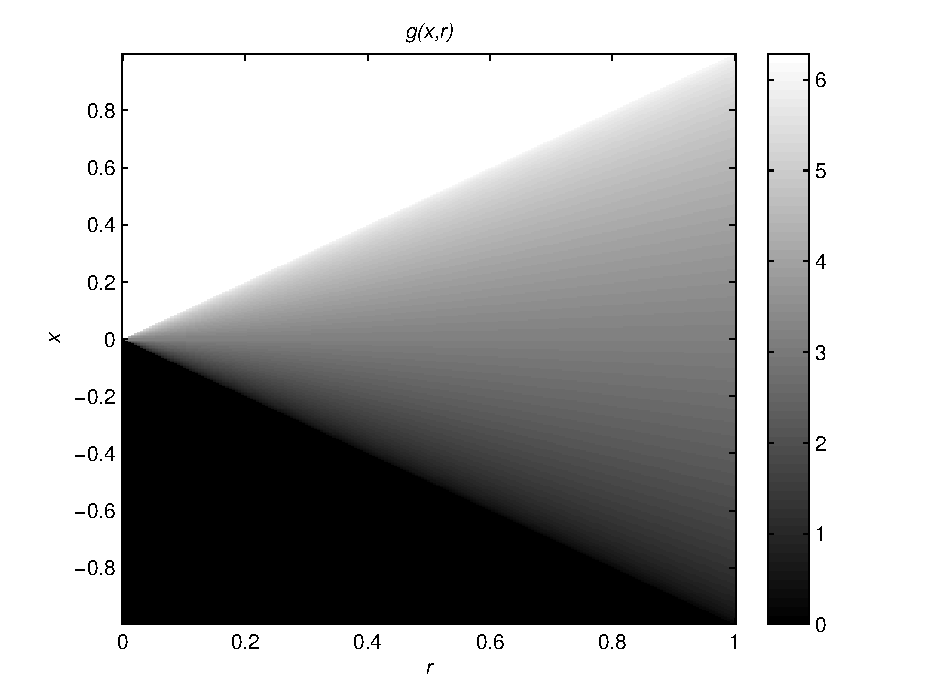
\includegraphics[width=.5\textwidth]{figures/g_function.pdf}

  Observe that $g$ is symmetric about $x=0$.
  \end{center}
  }
\end{frame}

%\begin{frame}[t]
%  \frametitle{A Synthetic Example}
%  A radially symmetric two-dimensional \alert{Gaussian PSF} has the form
%  \begin{equation*}
%    p(r) = (2\pi\sigma^2)^{-1} e^{\frac{-r^2}{2\sigma^2}} 
%  \end{equation*}
%  and it can be shown analytically that the analytic forward blur is an \alert{error function}
%  \begin{equation*}
%    [\mathcal G p] (x_i) = \frac 1{\sqrt{2\pi}\sigma} \int_{-\infty}^{x_i} e^{-\frac{s^2}{2\sigma^2}}\,ds
%  \end{equation*} 
%  \begin{tikzpicture}[pic/.style={inner sep=0pt,above right}]
%    \node[pic] at (-1,2.5) (left)     { \includegraphics[width=.4\textwidth]{figures/radial_gaussian_psf.pdf} };
%    \node[pic] at (5,2.5) (right)     { \includegraphics[width=.4\textwidth]{figures/radial_gaussian_edgeblur.pdf} };
%    \path[bend left,-latex] (3,6) edge node[above]{$\mathcal G$} (6,6); 
%  \end{tikzpicture}
%\end{frame}
%
\begin{frame}
  \frametitle{Radial Profile Inverse Problem}
  For the inverse problem
  \begin{equation*}
    b = \mathcal G p + \eps,
  \end{equation*}
  \begin{itemize}
%    \item $\mathcal G$ is a compact Hilbert-Schmidt operator, hence its inverse is unbounded.
    \item Hence, the discretized problem $\vect G \vect p = \vect b$ results in an ill-conditioned a matrix 
    \item The \alert{SVD} of a matrix: $\vect G = U \Sigma V^*$, so the left-inverse is $\vect G^\dagger = V \Sigma^\dagger U^*$.
  \end{itemize}
  \hspace{-2.5em}
  \includegraphics[width=.39\textwidth]{figures/g_singular_values.pdf}
  \includegraphics[width=.39\textwidth]{figures/g_singular_vectors.pdf}
  \includegraphics[width=.39\textwidth]{figures/g_least_squares.pdf}
\end{frame}

%\begin{frame}
%  \frametitle{Tikhonov Laplacian Regularization}
%  {\footnotesize For the two representations }
%  \begin{equation*}
%    b = \mathcal G p + \epsilon\quad\text{ and }\quad b= \mathcal F k + \epsilon
%  \end{equation*}
%  {\footnotesize
%%  regularization and uncertainty quantification can be achieved by modeling the PSF as a random quantity with an appropriate prior.
%  \begin{itemize}
%    \itemsep 1.2em
%    \item Minimizing the second order Tikhonov-Laplacian functional subject to $k$ radially symmetric
%    $$ \frac \lambda 2 \Big\|b - \G p\Big\|_{L^2}^2 + \frac \delta 2 \left\|\nabla^2 k\right\|_{L^2}^2  $$
%%    \item is equivalent to minimizing 
%%    $$ \frac \lambda 2 \Big\|b - \G p\Big\|_{L^2} + \frac \delta 2 \alert{\Big\|\LL p\Big\|_{rad}}  $$
%  \end{itemize}
%  }
%\end{frame}

%\subsection{Regularization and Discrete representation}
%\begin{frame}
%  \frametitle{Radial $L^2$ and the Laplacian}
%  {\footnotesize For the two representations }
%  \begin{equation*}
%    b = \mathcal G p + \vect \epsilon\quad\text{ and }\quad b= \mathcal F k + \vect \epsilon
%  \end{equation*}
%  {\footnotesize
%%  regularization and uncertainty quantification can be achieved by modeling the PSF as a random quantity with an appropriate prior.
%  \begin{itemize}
%    \itemsep 1.2em
%    \item The Laplacian on $\RR^2$  with the $L^2$ inner product
%      $$ \nabla^2 k \eqdef \left(\frac{\del^2}{\del x^2} + \frac{\del^2}{\del y^2}\right) k$$ 
%       is equivalent to the differential operator 
%      $$ \ds{\LL p \eqdef \frac1r \frac{d}{dr} \left(r \frac d{dr} p\right)} $$ 
%      with the inner product $\ds{(p,q)_{rad} = \int p(r)\cdot \bar q(r)\, \alert{r dr}}$.
%    \item We solve the inverse problem on the \alert{radial profile p}, with regularization on the \alert{radially symmetric function k}.
%    \item These notions can be made rigorous through the theory of \alert{distributions}.
%%    \item We use a \alert{Gaussian prior} defined implicitly on $k(s,t)$. Denote $\Delta^2_0$ as the squared Laplacian defined on a certain subspace of $L^2(\RR^2)$, then the prior density satisfies \alert{$\mathrm E\, \Delta^2_0 k = 0$} and \alert{$\mathrm{Var}\,\Delta^2_0 k = \delta^{-1} I$} \cite{stuart13bayesian}.
%%    \item For the polar coordinate map $T(r,\theta)$, the radial symmetry assumption gives $\displaystyle{(\mathcal L p)(r) := (\Delta^2_0 k \circ T)(r) = \alert{\left(\frac{1}{r} \frac{d}{dr} r\frac{d}{dr}\right)^2 p(r)}}$. Here, we impose a left zero derivative and right zero boundary condition on \alert{$p$}.
%  \end{itemize}
%  }
%\end{frame}
%\begin{frame}
%  \frametitle{Tikhonov Laplacian Regularization}
%  {\footnotesize For the two representations }
%  \begin{equation*}
%    b = \mathcal G p + \epsilon\quad\text{ and }\quad b= \mathcal F k + \epsilon
%  \end{equation*}
%  {\footnotesize
%%  regularization and uncertainty quantification can be achieved by modeling the PSF as a random quantity with an appropriate prior.
%  \begin{itemize}
%    \itemsep 1.2em
%    \item Minimizing the second order Tikhonov-Laplacian functional subject to $k$ radially symmetric
%    $$ \frac \lambda 2 \Big\|b - \G p\Big\|_{L^2}^2 + \frac \delta 2 \left\|\nabla^2 k\right\|_{L^2}^2  $$
%    \item is equivalent to minimizing 
%    $$ \frac \lambda 2 \Big\|b - \G p\Big\|_{L^2}^2 + \frac \delta 2 \alert{\Big\|\LL p\Big\|_{rad}^2}  $$
%  \end{itemize}
%  }
%\end{frame}
\begin{frame}
  \frametitle{The discrete problem}
  {\footnotesize 
  In order to carry out estimation on a computer, we discretize the integral operator using \alert{mid-point quadrature}}
  $$
    b = \mathcal G p + \epsilon\quad \implies \quad \vect b = \vect G \vect p + \vect\epsilon
  $$
  {\footnotesize  Further, we discretize the regularization operator $\LL$ using \alert{finite differencing} }
%  regularization and uncertainty quantification can be achieved by modeling the PSF as a random quantity with an appropriate prior.
    $$ 
      \ds{\|\LL p\|_{rad}^2 = \int \left[\frac1r \frac{d}{dr} \left(r \frac d{dr} \right)\right]^2 p(r) rdr}
      \implies 
      \vect L \vect p = \vect r^{-1/2} \odot \vect D \left(\vect r \odot \vect D\vect p\right) 
    $$
    {\footnotesize and \alert{midpoint quadrature} for the inner products
    \begin{align*}
      \frac \lambda {2} \Big\|b - \G p\Big\|_{L^2}^2 &\implies \alert{\underbrace{\frac \lambda {2m}}_{\ds{\lambda}}} \Big\|\vect b - \vect G \alert{\vect p}\Big\|_{\R^m}^2 \\ 
      \intertext{ and }
      \frac\delta2 \Big\|\nabla^2 k\|_{L^2} \implies \frac \delta {2} \Big\|\LL p\Big\|_{rad}^2  &\implies \alert{\underbrace{\frac \delta {2n}}_{\ds{\delta}}} \Big\|\vect L  \alert{\vect p}\Big\|_{\R^n}^2  
    \end{align*}
    }
\end{frame}

\section{Markov Chain Monte Carlo methods for posterior inference}
\subsection{Introduction to Monte Carlo estimation}
\begin{frame}
  \frametitle{Buffon's Needle}
    \begin{tikzpicture}[pic/.style={inner sep=0pt,above right}]
    \foreach \y in {0,2,4}{
      \draw (0,\y) -- (10,\y); 
    }
    \node[inner sep=0,outer sep=0] (pt) at (1,1) {};
    \node[inner sep=0,outer sep=0] (pin) at ([shift=(45:2)] pt) {};
    \draw[*-,blue] (pin) -- (pt);
    \end{tikzpicture}

    \begin{itemize}
    \itemsep 1.2em
      \item  Suppose a needle of unit length is dropped on a panelled floor with unit width panels.
      \item What is the probability that the needle crosses a panel line?
%      \item and $Y = \sin\Theta$.
    \end{itemize}
\end{frame}

\begin{frame}
  \frametitle{Buffon's Needle}
    \begin{tikzpicture}[pic/.style={inner sep=0pt,above right}]
    \foreach \y in {0,2,4}{
      \draw (0,\y) -- (10,\y); 
    }
    \node[inner sep=0,outer sep=0] (pt) at (1,1) {};
    \node[inner sep=0,outer sep=0] (pin) at ([shift=(45:2)] pt) {};
    \draw[*-,blue] (pin) -- (pt);
    \draw[dotted] (0,1) -- (10,1);
    \draw[blue] ([shift=(0:.3)] pt) arc (0:45:.3) node[right] {$\Theta$};
    \end{tikzpicture}

    \begin{itemize}
    \itemsep 1.2em
      \item{$C = 1$ if the needle crosses and 0 otherwise,}
      \item{Let $\Theta$ be the angle the bottom point of the needle makes with the horizontal,}\\
    \end{itemize}
\end{frame}

\begin{frame}
  \frametitle{Buffon's Needle}
    \begin{tikzpicture}[pic/.style={inner sep=0pt,above right}]
    \foreach \y in {0,2,4}{
      \draw (0,\y) -- (10,\y); 
    }
    \node[inner sep=0,outer sep=0] (pt) at (1,1) {};
    \node[inner sep=0,outer sep=0] (pin) at ([shift=(45:2)] pt) {};
    \draw[*-,blue] (pin) -- (pt);
    \draw[dotted] (0,1) -- (10,1);
    \draw[blue] ([shift=(0:.3)] pt) arc (0:45:.3) node[right] {$\Theta$};
    \draw[blue] ( pin) -- node[right] {$\sin \Theta$} ++(0,-1.414);
    \end{tikzpicture}

    \begin{itemize}
    \itemsep 1.2em
      \item{$\ds{\PP(C = 1 | \Theta = \theta) = \sin\theta }$ and $\ds{\PP(C = 0 | \Theta = \theta) = 1 - \sin\theta }$.}
      \item{$\ds{\PP(\Theta = \theta ) = \frac1\pi I_{[0,\pi]}(\theta) }$ where $I_S$ is the indicator function for $S$.}
%      \item<only@1>{$C = 1$ if the needle crosses and 0 otherwise,}
%      \item<only@1>{Let $\Theta$ be the angle the bottom point of the needle makes with the horizontal,}\\
%      \item<only@2>{$\ds{\PP(\Theta = \theta ) = \frac1\pi I_{[0,\pi]}(\theta) }$ where $I_S$ is the indicator function for $S$.}
%      \item<only@2>{$\ds{\PP(C = 1 | \Theta = \theta) = \sin\theta }$ and $\ds{\PP(C = 0 | \Theta = \theta) = 1 - \sin\theta }$.}
%      \item and $Y = \sin\Theta$.
    \end{itemize}
\end{frame}

\begin{frame}[t]
  \frametitle{Bayes' ``Theorem''}
    \begin{itemize}
    \itemsep 1.2em
      \item Bayes:\\ (i) $\ds{\PP(A = a| B = b)\PP(B = b) = \PP(A = a, B = b)}$ \\ (ii) $\int \PP(A = a, B = b)db = \PP(A = a)$.
%      \item $\ds{\PP(Y = y |  \alert{C =1}, \Theta = \theta ) \PP(\alert{C = 1} | \Theta = \theta ) }$\\ $\quad= \PP(Y = y , \alert{C =1}| \Theta = \theta )$ 
      \item $\ds{\PP(C =1| \alert{\Theta = \theta} ) \PP(\alert{\Theta = \theta }) } = \PP(C =1, \alert{\Theta = \theta} )$ 
    \end{itemize}
    So,
    \begin{align*}
      \PP( C =1, \Theta = \theta ) 
        &= \frac1\pi I_{[0,\pi]}(\theta) \cdot \sin\theta \\
%        &= \frac1\pi I_{[0,\pi]}(\theta)I_{[0,\sin\theta]}(\theta)
    \end{align*}
    and
        $$\PP(C =1) = \int \PP(C=1,\theta) d\theta = \int_0^\pi\frac{\sin \theta}\pi d\theta = \frac 2\pi$$
\end{frame}
\begin{frame}
  \frametitle{Buffon's Monte Carlo Needles}
  \includegraphics[height=.8\textheight]{figures/needledrop.pdf}

  \begin{itemize}
  \item<only@1>{Drop \color{blue}{$N$} needles.}
  \end{itemize}
\end{frame}
\begin{frame}
  \frametitle{Buffon's Monte Carlo Needles}
  \includegraphics[height=.8\textheight]{figures/needledropcount.pdf}

  \begin{itemize}
  \item<only@1>{Let $\alert{\{C_1,\dots C_{N}\}}$ be the simulated needle crossings.}
  \item<only@2>{The Law of Large Numbers says $2 \textcolor{blue}{N} / \alert{\sum C_i} \to \pi$.}
  \item<only@3>{The Strong Law of Large Numbers says $\sigma$ for $\frac 1N \sum C_i$ is $O( 1/\sqrt{N} )$.}
  \item<only@4>{So for $N = 100$, $\pi \approx 200/67 \approx 2.9851$ with $\sigma = O(10^{-1})$.}
  \end{itemize}
\end{frame}

\subsection{The posterior density}
\begin{frame}[t]
  \frametitle{Hierarchical Model for PSF estimation}
  Let $\pi(\vect x) = \PP(X = x)$ denote the probability density. For $\lambda,\delta$ and $\vect p$ and
  $$\vect b = \vect G \vect p + \vect \epsilon$$
  assume
  \begin{itemize}
    \itemsep 1.2em
    \item The \alert{likelihood} $\alert{\pi(\vect b|\vect p,\lambda,\delta) = \pi(\vect b| \vect p,\lambda) \propto \lambda^{M/2}\exp\left(-\frac\lambda2 \|\vect b - \vect G\vect p\|^2\right)}$ since $\vect \epsilon$ is independent Gaussian noise.
    \item The \alert{prior} \alert{$\pi(\vect p| \delta,\lambda) = \pi(\vect p| \delta) \propto \delta^{N/2}\exp\left(-\frac \delta{2} \|\vect L \vect p\|^2\right)$} since $k \sim \N(0,\nabla^{-2}) \implies p\sim N(0,\LL^{-2})$ 
    \item The \alert{hyperpriors} \alert{$\pi(\lambda) \propto \exp\left(-10^{-4}\lambda\right)$} and \alert{$\pi(\delta) \propto \exp\left(-10^{-4} \delta\right)$} are independent ``unobjective'' Gamma distributions.
  \end{itemize}
\end{frame}
\newcommand{\pib}{\pi_{\mathbf b}}
\begin{frame}[t]
  \frametitle{Bayesian Posterior}
  With $\pi(\vect b|\vect p,\lambda,\delta),\pi(\vect p| \delta,\lambda),$ and $\pi(\lambda,\delta)$, use Bayes' ``Theorem'' to obtain
  {\small
  \begin{align*}
    \pib(\alert{\vect p,\lambda,\delta}) &\eqdef \pi(\alert{\vect p,\lambda,\delta}|\vect b) = \pi(\vect b,\vect p,\lambda,\delta)/\pi(\vect b) \\
      &\propto {\alert{\lambda}}^{M/2}\alert{{\delta}}^{N/2}\exp\left(
        -\frac {\alert{\lambda}}{2} 
        \Big\|\vect b - \vect G \alert{\vect p}\Big\|_{\R^m} - \frac {\alert{\delta}} 2\Big\|\vect L  \alert{\vect p}\Big\|_{\R^n} - 10^{-4}(\alert\lambda + \alert\delta)
        \right) 
  \end{align*}
  }
  \begin{itemize}
    \itemsep 1.2em
    \item This is not a ``common'' probability density, hence simulations from a computer are not readily available.
    \item Leveraging conditional density ideas will give us a method to simulate a Monte Carlo method like Buffon's needle problem.
    \item Bayes' ``Theorem'' will allow simulations from the \alert{full conditionals} $\pib(\lambda|\delta,\vect p), \pib(\delta|\lambda,\vect p)$ and $\pib(\vect p|\lambda,\delta)$.
  \end{itemize}
\end{frame}

\subsection{Gibbs Sampling}
\begin{frame}[t]
  \frametitle{Markov Chains}
{\small
  \begin{itemize}
  \itemsep 1.2em
  \item A \alert{transition operator} is a linear map on probability densities $\pi$, so that
    $$
      \K [\pi](\vect x') = \int K(\vect x,\vect x') \pi(\vect x)d\vect x. 
    $$
  where $K(\vect x,\cdot)$, the \alert{transition kernel}.%, if for all $\vect x \in \R^M$, $K(\vect x,\cdot)$, it defines a probability measure given by 

  \item A \alert{Markov chain} is a stochastic process $\{\vect X^0, \vect X^1,\vect X^2,\dots,\}$ with $\vect X^k:\Omega \to \R^M$ such that %defined on a common probability space such that for a given transition kernel $K$,
  \begin{align*}
  \mathbb P\left( \vect X^{k+1} = x^{k+1} | \vect X^k= \vect x^k,\dots,\vect X^0=\vect x^0\right) 
    &= \mathbb P\left( \vect X^{k+1} = \vect x^{k+1} | \vect X^k= \vect x^k\right) \\
    &= K(\vect x^k,\vect x^{k+1}).
  \end{align*}
  So, given an initial density $\pi_0({\vect x}^0)$
  $$
    \PP( \vect X^N = {\vect x}^N ) = \K^N[\pi_0]({\vect x}^N)
  $$
  \item Markov chains are \alert{not independent} and \alert{not identically distributed}. 
%for all events $A$, i.e., the random variable $\vect X^{k+1}$ depends only on the previous realization $\vect X^k=\vect x^k$, and subsequent densities of the elements in the Markov Chain are given by the action of the transition operator.
\end{itemize}
}
\end{frame}

\begin{frame}[t]
  \frametitle{An Ergodic Theorem}

  {\bf Theorem}[Tierney1994]: Suppose $\K$ defines a \alert{stationary} Markov chain with \alert{invariant} density $\pi$. If the chain is \alert{$\pi$-irreducible} and \alert{Harris recurrent}, then $\pi$ is unique and for any initial density $\pi_0$ and all $\vect x$ but a subset whose measure under $\pi$ is zero. Moreover,
  \begin{enumerate}[(i)]
    \item Almost surely with respect to $\pi$, for any integrable $h$ \begin{equation} \lim_{N\to \infty}\frac 1N\sum_{n=1}^N h(\vect X^n) = \int h(\vect x) \pi(\vect x) d\vect x. \label{eq:ergodicStat}\end{equation}
    \item If in addition, the chain is \alert{aperiodic}, then $$\lim_{N\to \infty}\|\K^N\pi_0 - \pi\|_{TV} = 0,$$ 
    where $\|\pi\|_{TV}$ denotes the supremum of $\int_A \pi(x) dx$ over all Borel sets $A$.
  \end{enumerate}
\end{frame}

\begin{frame}[t]
  \frametitle{Ergodic Theorem Hypotheses}
  \begin{itemize}
    \itemsep 1.2em
    \item A Markov chain is \alert{stationary} and \alert{invariant} with respect to $\pi$ if \alert{$\K \pi = \pi$}.
    \item \alert{MCMC idea:} Design a Markov chain that has $\pib(\alert{\vect p,\lambda,\delta})$ as its invariant density, i.e.~$\K \pib = \pib$.
    \item \alert{Harris recurrence , irreducibility, and aperiodicity} are necessary conditions so ensure that the evolution of the chain ``explores'' the invariant density $\pi$ enough and avoids transient states.
    \item The first step to appealing to the ergodic theorem is to ensure \alert{invariance} with the desired density.
  \end{itemize}
\end{frame}

\begin{frame}[t]
  \frametitle{MCMC Inference by the Ergodic Theorem}
  \begin{itemize}
    \itemsep 1.2em
    \item The first conclusion of the Ergodic theorem says that \alert{statistics} on the realizations of the chain converge as expected.
    \item The second conclusion is \alert{distributional}, and implies that late stages in the chain are ``approximately'' \alert{identically distributed}, but \alert{not independent}.

    \includegraphics[width=.8\textwidth]{figures/psf_hierarchical_chains_1000.pdf}\\
  \end{itemize}
\end{frame}

\begin{frame}[t]
  \frametitle{Gibbs sampling}
{\small
  The Gibbs sampler [Geman and Geman 1984]: 
  
Given $\left(\lambda^{k-1},\delta^{k-1},\vect p^{k-1}\right)$, simulate
\begin{center}
\begin{algorithmic}[1]
  \STATE $\lambda^k \sim \alert{\pib(\lambda|\delta^{k-1},\vect p^{k-1})}$
  \STATE $\delta^{k} \sim \color{blue}{\pib(\delta|\lambda^k,\vect p^{k-1})}$ 
  \STATE $\vect p^{k} \sim \pib(\vect p|\lambda^k,\delta^k)$
\end{algorithmic}
\end{center}

}
The associated Markov Chain is invariant with respect to $\pi$:
{\footnotesize
\begin{align*}
[\K\pib](\lambda',\delta',\vect p') 
\pause  &= \iiint \pib(\vect p'|\lambda',\delta') \textcolor{blue}{\pib(\delta'|\lambda',\vect p)}\alert{\pib(\lambda'|\delta,\vect p)}\pib(\lambda,\delta,\vect p)d\lambda d\delta d\vect p \\
\pause  &= \pib(\vect p'|\lambda',\delta')\int \textcolor{blue}{\pib(\delta'|\lambda',\vect p)}\int\alert{\underbrace{\pib(\lambda'|\delta,\vect p)}_{\pib(\lambda',\delta,\mathbf p)/\pib(\delta,\mathbf p)}}\int\pib(\lambda,\delta,\vect p)d\lambda d\delta d\vect p \\
\pause  &= \pib(\vect p'|\lambda',\delta')\int \textcolor{blue}{\underbrace{\pib(\delta'|\lambda',\vect p)}_{\pib(\lambda',\delta',\mathbf p)/\pib(\lambda',\mathbf p)}}\int \pib(\lambda',\delta,\vect p)d\delta d\vect p \\
\pause  &\dots \\
\pause  &= \pib(\vect p',\lambda',\delta'),\text{ so the Gibbs sampler is invariant.}
\end{align*}
}
\end{frame}


\begin{frame}[t]
  \frametitle{Correlated $\delta$ chains}
  \vspace{-1.2em}
  \begin{center}
    \includegraphics[width=.8\textwidth]{figures/psf_hierarchical_chains_50.pdf}\\
    \includegraphics[width=.8\textwidth]{figures/psf_hierarchical_chains_1000.pdf}\\ 
    %\includegraphics[width=.5\textwidth]{figures/psf_hierarchical_autocor_50.pdf}  \includegraphics[width=.5\textwidth]{figures/psf_hierarchical_chains_50.pdf}\\
    %\includegraphics[width=.5\textwidth]{figures/psf_hierarchical_autocor_500.pdf} \includegraphics[width=.5\textwidth]{figures/psf_hierarchical_chains_500.pdf}\\ 
    %\includegraphics[width=.5\textwidth]{figures/psf_hierarchical_autocor_1000.pdf} \includegraphics[width=.5\textwidth]{figures/psf_hierarchical_chains_1000.pdf}\\ 
  \end{center}
\end{frame}

\subsection{Collapsing the Gibbs Sampler}
\begin{frame}[t]
  \frametitle{Literature on the Issue}
  {\small
  \begin{itemize}
    \itemsep 1.2em
    \item \,[Agapiou,Bardsley,Stuart,Papaspiliopoulos, 2014] explained this phenomena theoretically for a general class of Laplacian based Hierarchical samplers for inverse problems.
    \item The issue arises when the discretization of \alert{$\vect p$} closer approximates the continuum, the correlation in the \alert{$\delta$} component of the Markov Chain becomes more correlated.
    \item \,[VanDyke, Park 2008] provide a general method for removing the dependence of problematic components in the Gibbs sampler, called \alert{partial collapse}.
    \item The idea has been independently derived in many places, however, if done carelessly [VanDyke, Park 2008] showed that the resulting Markov chain is no longer \alert{invariant}, although invariance was not proved there.
  \end{itemize}
  }
\end{frame}

\begin{frame}[t]
  \frametitle{Marginalized Sampler}
{\small
Given $\left(\lambda^{k-1},\delta^{k-1},\vect p^{k-1},\alert{\tilde{\vect p}^{k-1}}\right)$, simulate
\begin{center}
\begin{algorithmic}[1]
  \STATE $\lambda^k \sim \pib(\lambda|\delta^{k-1},\vect p^{k-1})$
  \STATE \textcolor{blue}{$(\delta^{k},\alert{\tilde{\vect p}^k}) \sim \pib(\delta,\alert{\tilde{\vect p}}|\lambda^k)$}
  \STATE \textcolor{blue}{$\vect p^{k} \sim \pib(\vect p|\lambda^k,\delta^k)$}
\end{algorithmic}
\end{center}
The associated Markov Chain is invariant with respect to $\tilde \pib(\lambda,\delta,\vect p,\tilde{\vect p}) = \alert{\pib(\lambda,\delta,\vect p)\pib(\tilde{\vect p}| \lambda,\delta)}$:  
}
{\footnotesize
\begin{align*}
 [\K\tilde\pib] 
\pause   &= \iiiint  \textcolor{blue}{\pib(\vect p'|\lambda',\delta')\pib(\delta',\tilde{\vect p}'|\lambda')}\pib(\lambda',\vect p|\delta)\alert{\tilde \pib(\lambda,\delta,\vect p,\tilde{\vect p})}d\lambda d\delta d\vect p d\tilde{\vect p} \\ 
\pause   &= \textcolor{blue}{\pib(\vect p'|\lambda',\delta')} \textcolor{blue}{\pib(\delta',\tilde{\vect p}'|\lambda')}\iint {\pib(\lambda'|\delta,\vect p)}\underbrace{\int\alert{\int \tilde \pib(\lambda,\delta,\vect p,\tilde{\vect p}) d\tilde{\vect p}}d\lambda }_{\pib(\delta,\mathbf p)}d\delta d\vect p \\
\pause   &= \textcolor{blue}{\underbrace{\pib(\vect p'|\lambda',\delta')}_{\pib(\mathbf p',\delta',\lambda')/\pib(\delta',\lambda')} \pib(\delta',\tilde{\vect p}'|\lambda')}\underbrace{\iint \pib(\lambda',\delta,\vect p) d\delta d\vect p}_{\pib(\lambda')} \\
\pause   &= \pib(\vect p',\lambda',\delta') \frac{\pib( \tilde {\vect p}',\lambda',\delta')}{\pib(\lambda',\delta')} \\
\pause   &= \tilde \pib(\lambda',\delta',\vect p',\tilde{\vect p}')
\end{align*}
}
\end{frame}

\begin{frame}[t]
  \frametitle{Partially Collapsed Sampler}
{\small
Given $\left(\lambda^{k-1},\delta^{k-1},\vect p^{k-1}\right)$, simulate
\begin{center}
\begin{algorithmic}[1]
  \STATE $\lambda^k \sim \pib(\lambda|\delta^{k-1},\vect p^{k-1})$
  \STATE $\delta^{k} \sim \pib(\delta|\lambda^k)$ 
  \STATE $\vect p^{k} \sim \pib(\vect p|\lambda^k,\delta^k)$
\end{algorithmic}
\end{center}
The associated Markov Chain is invariant with respect to $\int \tilde \pib(\lambda,\delta,\vect p,\tilde{\vect p}) = \int \pib(\lambda,\delta,\vect p)\pib(\tilde{\vect p}| \lambda,\delta) = \pib(\lambda,\delta,\vect p)$.
}

\begin{itemize}
  \itemsep 1.2em
  \item The order of the chain matters in the previous arguments.
  \item \alert{Permuting} steps 2 and 3 results in a chain that is no longer \alert{invariant} with respect to $\pib$.
  \item \alert{Cyclically permuting} results in a different sampler as well, however, this does not practically effect the overall chain, only the first and last steps, e.g. $(\K_1\K_3\K_2)^N = \K_1\alert{(\K_3\K_2\K_1)^{N-1}}\K_2\K_3$
\end{itemize}
\end{frame}
\begin{frame}[t]
\frametitle{Marginalized Posterior Density}
{\footnotesize
In order to sample $\pib(\delta|\lambda)$, we \alert{complete the square} of the quadratic form in $\pib(\lambda,\delta,\vect p)$ and integrate out $\lambda$, this results in
  \begin{align*}
    \pib( \delta|\lambda) 
    &\propto\exp\left( (n/2)\delta -  \alert{\ln |\det \vect J_{\lambda,\delta}|}  - \alert{\frac \lambda 2 \langle\vect b, \vect H_{\lambda,\delta}\vect b \rangle}  -10^{-4}\delta \right),
  \end{align*}
  where \alert{$\vect J_{\lambda,\delta} = \lambda \vect G^T\vect G + \delta \vect L$ and $\vect H_{\lambda,\delta} = \vect I - \lambda \vect G\vect J_{\lambda,\delta}^{-1}\vect G^T$}.
\begin{itemize}
\itemsep 1.2em
  \item To draw from this density, we embed a \alert{Metropolis-Hastings} algorithm within the Gibbs sampler.
  \item It can be shown that the resulting MCMC algorithm remains invariant.
  \item Both constants can be carried out using a Cholesky factorization \alert{$\vect R_{\lambda,\delta}^T \vect R_{\lambda,\delta} = J_{\lambda,\delta}$} in ($O(n^3)$) flops, and will be required for each Metropolis step. 
\end{itemize}
}
\end{frame}

\begin{frame}[t]
  \frametitle{Metropolis-Hastings within Gibbs Sampling}
  {\footnotesize
  \begin{itemize}
    \itemsep 1.1em
    \item We use $n_{MH}$ \alert{Metropolis-Hastings} steps using a Gaussian proposal with variance $\gamma$.
    \item Due to numerical overflow issues, all computations are carried out on the log scale.
    \item The full implementation is:
  \end{itemize}
  \begin{algorithmic}[1]
  \STATE Let $\lambda_0$, $\delta_0$,$\vect p$ and $\gamma$ be given.
  %STATE   \item Draw $\vect z_k$ from  $N(0,\vect I)$, and compute $\vect p_k = \vect S_k^{-1}(\vect z_k + \vect {S_k^T}^{-1}\lambda_k \vect A^T \vect b)$.
  \STATE Draw $\lambda_{k+1}$ from $\Gamma \Big(n/2+\alpha,\,\frac12\|\vect{Ax_k} - \vect b\|^2 - \beta \Big)$.
  %\STATE Compute $\vect {J_k} = \vect{R_k}^T \vect{R_k}$. 
  \STATE Set $j = 1$, Compute \alert{$\vect R_0^T \vect R_0  = \vect J_{\lambda^k,\delta^{k-1}}$, then $\pi_0 = \log \pib(\delta^{k-1}|\lambda^k)$}.
  \FOR{$1<j<n_{MH}$} 
    \STATE Draw $\tilde \delta$ from $N(\tilde \delta_{j-1}, \gamma)$.
    \STATE Compute \alert{$\tilde{\vect R}^T\tilde{\vect R} = J_{\lambda^k,\tilde \delta}$, then $\pi_j = \log p(\tilde \delta_j|\vect f \lambda _k)$}.
    \STATE Set $\tilde \pi = \pi_j, \vect R_j = \tilde{\vect R}$ and $\delta_{k} = \tilde \delta_j$ with probability $\tilde \pi/\pi_j$
  \ENDFOR
  \STATE Draw $\vect p_k$ from $N\Big( \vect R_k^{-1}\lambda_k \vect A^T\vect b, \vect R_k^{-1} \Big)$.
  \STATE Set $k=k+1$ and return to 2.
  \end{algorithmic}
  }
\end{frame}

\subsection{Results}

\begin{frame}[t]
  \frametitle{Marginalized $\delta$ chains}
  \vspace{-1.2em}
  \begin{center}
    \includegraphics[width=.8\textwidth]{figures/psf_marginalized_chains_50.pdf}\\
    \includegraphics[width=.8\textwidth]{figures/psf_marginalized_chains_1000.pdf}\\ 
  \end{center}
\end{frame}

\begin{frame}[t]
  \frametitle{Results}
\makebox[\textwidth][c]{
  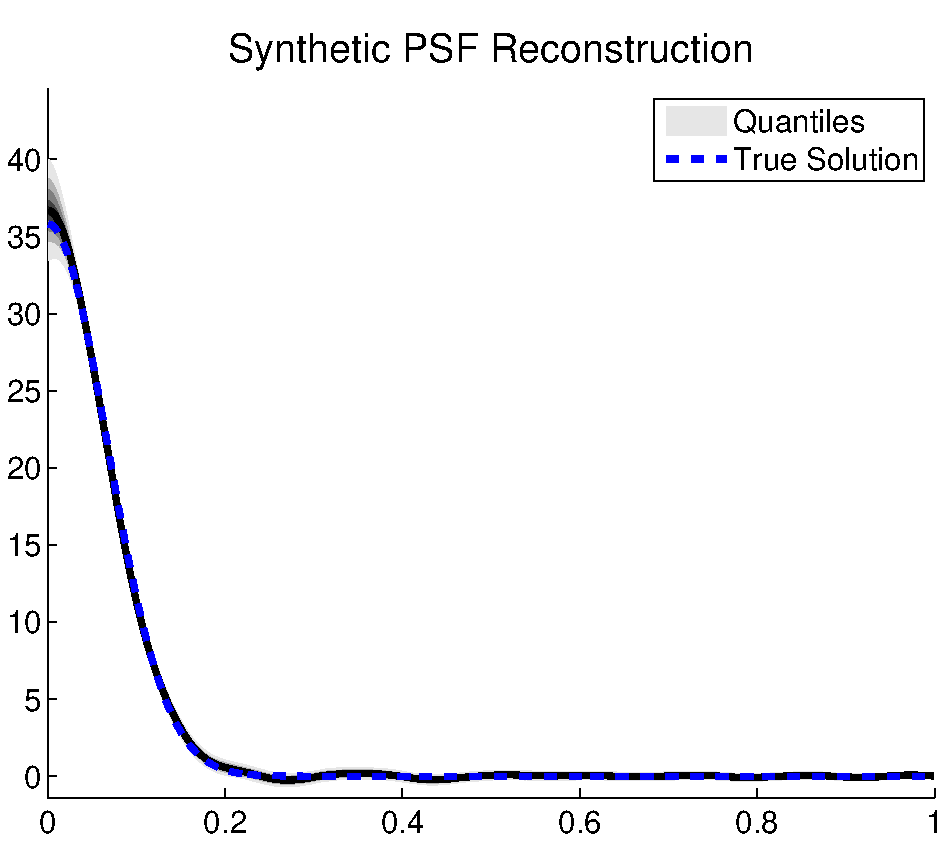
\includegraphics[width=.45\textwidth]{partially_collapsed_gibbs/syntheticPSFrecon.pdf}
  \includegraphics[width=.6\textwidth]{figures/marginalized_pdf_psf_recon.pdf}
}

\vspace{3em}

{\tiny
  \begin{tabular}{l|ccccccc}
    \hline
% Jan. 9 values initial delta = 1 and initial lambda = 1
    Algorithm       & $\hat{\lambda}_{\rm MCMC}$& $\hat{\delta}_{\rm MCMC}$  & $\lambda$-$p_{\rm Geweke}$&$\delta$-$p_{\rm Geweke}$& IACT & ESS    & \#Chol/ESS \\
     & $(\times 10^{4})$ & ($\times 10^{-8}$) & & \\
    \hline
   Gibbs &                 1.102 &                 6.132 &                   0.998 &                    0.850& 36.2 &  138.0 &      \alert{72.4} \\
PC Gibbs &                 1.102 &                 5.611 &                   0.992 &                    0.943&  7.9 &  633.0 &      \alert{31.6} \\
\hspace{.2in} $n_{mh}= 1$ & & & & & & & \\
PC Gibbs &                 1.102 &                 5.515 &                   0.999 &                    0.985&  1.3 & 3799.6 &      \alert{15.8} \\
\hspace{.2in} $n_{mh}= 5$ & & & & & & & \\
%     MTC &                 1.099 &                 5.419 &                   0.998 &                    0.934& 11.5 &  473.2 &      21.1 \\
    % Dec. 11 values initial delta = norm(B) and initial lambda = 1/var( b(1:10) )
%    Gibbs             &                   0.997 &                    0.850& 46.3 &  107.9 &      92.6 \\
%    PC Gibbs $m_h=1$  &                   0.999 &                    0.955&  5.2 &  954.6 &      21.0 \\
%    PC Gibbs $m_h=5$  &                   0.998 &                    0.981&  1.7 & 2981.8 &      20.1 \\
%    MTC               &                   0.990 &                    0.950& 11.3 &  443.3 &      22.6 \\
    \hline
  \end{tabular}
}

\end{frame}

\begin{frame}[t]
  \frametitle{Summary and Future Work}
  {\small
  \begin{itemize}
  \itemsep 1.2em
    \item We introduced a novel \alert{Hierarchical Bayesian non-parametric model} for estimating \alert{translation invariant} and \alert{isotropic} image blur with and edge.
    \item We developed the \alert{Partially Collapsed Gibbs sampler} from the Gibbs sampler, and showed when partial collapse remained \alert{stationary}.
    \item We then implemented the algorithm on a synthetic example using \alert{Metropolis with Partially Collapsed Gibbs}, and showed that it improves the standard Gibbs sampler.
    \item \alert{Future:} Develop the model and algorithm completely in infinite dimensions.
    \item \alert{Future:} Adapt the strategies to other imaging models that incorporate \alert{radial geometry} such as Abel and Radon transforms.
  \end{itemize}
  }
\end{frame}

\begin{frame}
  \frametitle{References}
  \bibliographystyle{alpha}
  {\footnotesize
  \bibliography{edge_spread}
  }
\end{frame}

\end{document}
